\documentclass{article}

% set font encoding for PDFLaTeX or XeLaTeX
\usepackage{graphicx}
\usepackage{ifxetex}
\ifxetex
  \usepackage{fontspec}
\else
  \usepackage[T1]{fontenc}
  \usepackage[utf8]{inputenc}
  \usepackage{lmodern}
\fi
\title{Actividad 6}
\author{Corral Valdez Jesus Giovanni\\
Departamento de Física
}

% Enable SageTeX to run SageMath code right inside this LaTeX file.
% documentation: http://mirrors.ctan.org/macros/latex/contrib/sagetex/sagetexpackage.pdf
% \usepackage{sagetex}

\begin{document}
\maketitle
\section{Rotación de la luna}
La luna terrestre también tiene un movimiento rotacional sobre la misma Tierra, meintras esta gira alrededor del sol. Este periodo tiene una duración de 27.3217 dias.

\section{Codigo del programa}
\begin{verbatim}
function solx(angsol) result (x)
	double precision, intent(in) :: angsol
	double precision 	     :: x
        double precision, parameter :: rsolar = 1.496d8
	 x = rsolar * dcos(angsol)
end function solx
function soly(angsol) result (y)
	double precision, intent(in) :: angsol
	double precision 	     :: y
	double precision, parameter :: rsolar = 1.496d8
	 y = rsolar * dsin(angsol)
end function soly

subroutine moon(rsolar, rlunar, posx, posy, anglun, angsol)
   double precision, intent (in) :: rsolar, anglun, angsol
   double precision, intent (out) :: posx, posy
   double precision :: rlunar
   rlunar = rsolar / 4.0d0
   posx = (rsolar * dcos(angsol)) +(rlunar * dcos(anglun))
   posy = (rsolar * dsin(angsol)) +(rlunar * dsin(anglun))
 
end subroutine moon 


program luna
	implicit none
	integer :: i
	double precision :: g, dia, rsolar, rlunar, posx, posy, anglun
	double precision :: rad, velocidadlun, velocidadsol, solx, soly, angsol
	double precision, parameter :: pi=3.1416d0, mes = 27.3217d0, year = 365.26d0
	double precision, dimension(360) :: totalx,totaly
	double precision, dimension(360) :: x, y
  rsolar = 1.496d8
  rad = pi / 180.0d0
  dia = 365.26d0/(360.0d0*rad) !para saber cuantos dias pasan por radian
  velocidadlun = 2.0d0 * (pi / mes) !Es lo que recorre diariamente la luna en radianes
  velocidadsol = 2.0d0 * (pi / year)  
  
open (1, file = 'Lunatierra.dat', status = 'unknown')
open (2, file = 'Tierrasol.dat', status = 'unknown')
 do i=1, 360, 1
 g = dble(i)
 angsol = g * velocidadsol
 anglun = g * velocidadlun  !para saber la posicion actual en radianes
 x(i) = solx(angsol)
 y(i) = soly(angsol) !Las posiciones dadas por la funcion, para la posicion de la tierra respecto al sol 
 call moon(rsolar, rlunar, posx, posy, anglun, angsol)  !para calcular la posicion de la luna respecto a la tierra y el sol
 totalx(i) = posx
 totaly(i) = posy
 write (1,*) totalx(i), totaly(i)
 write (1,*) ' '
 write (2,*) x(i), y(i)
 write (2,*) ' '
 
 end do
 close (1)
 close (2)
end program luna
   
 
 
\end{verbatim}
\clearpage
\section{Grafica de posición}
El proposito del programa fue esta grafca, que muestra el movimiento de traslación de la Tierra mientras una luna gira sobre ella.
\begin{figure}
  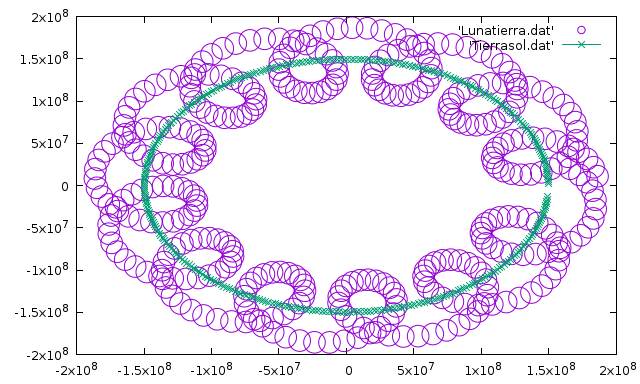
\includegraphics[width=\linewidth]{Sistema.png}
  \caption{Sistema Tierra-Luna-Sol}
\end{figure}


\end{document}
